% \iffalse

% \section{Additional Error Catching Evaluation}
% \label{app:snarkprobe-extraerror}

% We now discuss various inconsistency warnings that \tool automatically found during our evaluation.  While many of these are ``safe'' optimizations, we do not consider these warnings to be false positive results, as we want to flag both critical, exploitable errors, as well as subtle modifications that would benefit from expert review to ensure their safety.

% \subsection{\pinocchio Protocol Inconsistencies}
% In the \pinocchio key generator, values $\overrightarrow{A}$, $\overrightarrow{B}$, and $\overrightarrow{C}$ need to be extended via $A_{m+1} = B_{m+2} = C_{m+3}$ and $A_{m+2} = A_{m+3} = B_{m+1} = B_{m+3} = C_{m+1} = C_{m+2}$ as part of the specification \cite{ben2014succinct}. However, our \valuechecker found that \libsnark only extended $\overrightarrow{A}$, $\overrightarrow{B}$, and $\overrightarrow{C}$ via $A_{m+1} = B_{m+1} = C_{m+1}$ due to an optimization for space complexity, which our tool flagged because it does not match the original protocol specification. After a review of the \libsnark source code and protocol, we believe this inconsistency will not lead to a specific security vulnerability in \libsnark, but we believe that all inconsistencies between source code and protocol specification should be flagged and carefully reviewed, particularly for newer implementations that are not as battle-tested as \libsnark. This also serves as a demonstration that \SnarkFuzzer can indeed detect protocol inconsistencies in actual zkSNARK libraries, meaning that security engineers could utilize our tool to help focus their time and energy on the inconsistencies and potential issues that \tool found, which will reduce the time and cost for code auditing.

% Additionally, our \valuechecker also detected the \pinocchio protocol vulnerability reported as CVE-2019-7167 \cite{gabizon2019auroralight} in \libsnark.  This vulnerability was found by Gabizon in 2019 \cite{gabizon2019auroralight} and has since been fixed by Zcash \cite{zcash} and in \libsnark. At a high level, this vulnerability produced a bypass element in the key generation that damaged the soundness of the zkSNARKs proof system. To fix this vulnerability, the value of $pk_{A}^{'}$ will be replaced from $\{A_{i}(\tau)\alpha_{A}\rho_{A}\mathcal{P}\}_{i=0}^{m+3}$ to $\{A_{i}(\tau)\alpha_{A}\rho_{A}\mathcal{P}\}_{i=n+1}^{m+3}$, and other proving keys remain same. When running \SnarkFuzzer, the \valuechecker found this inconsistency in key generation. While \libsnark has fixed this issue, it did not directly modify the structure of proving key $pk_{A}^{'}$ in order to keep consistency with the structure of the other proving keys. Therefore, $pk_{A}^{'}$ still has size $m + 3$ instead of $(m + 3) - (n + 1)$. \libsnark added an extra handler to reformat the $pk_{A}^{'}$ size in the prover, but not following the original protocol still could bring risks that may break the soundness of the proof system.

% %%%%%

% \subsection{\groth16 Protocol Inconsistencies}
% The \groth16 protocol produces $P = g^{\alpha}$ and $Q = h^{\beta}$ as part of \textsf{Groth.Setup}, which are subsequently used in \textsf{Groth.Verify} to calculate the pairing $e(P, Q)$. However, our \valuechecker found that \libsnark uses the pairing of $e(P, Q)$ as part of the verification key in place of $P$ and $Q$ in \textsf{Groth.Setup}. Directly providing $e(P, Q)$ is an optimization that helps make verification more efficient (as pairings are quite slow to calculate).  As this is a well-known optimization, we can confidently say that this will not cause any sort of vulnerability, but again, we flag all inconsistencies between the source code and protocol for further review since not following the protocol can greatly increase the risk of cause cryptographic implementation errors.

% \fi

%%%%%%%%%%

\section{Additional Information for \ConstraintChecker}


\subsection{An Optimization for the SMT Solver}
\label{app:snarkprobe-constraintopt}

The SMT solver may take a while to solve some complicated equations. To reduce the processing time in the equality check, we introduce optimizations and simplify some equations in the R1CS matrix. For example, many \libsnark gadgets use bit shifting, which produces the equation $(x * (1 + (p - 1) * x)) \bmod p = 0$ in R1CS gates. This equation represents $x = 0$ or $x = 1$. For our optimization, if the \ConstraintChecker detects such a relation, it will be replaced with $0 \le x \land x \le 1$ where $x \in \mathbb{F}$. These are logically equivalent, but our replacement is much easier for the SMT solver to work with.  A real world gadget like the \texttt{comparison\_gadget} in \libsnark has 16 constraints, and there are 11 constraints representing $x = 0$ or $x = 1$ (see \autoref{eq:comparison_gadget}). %Therefore, this replacement optimization can significantly reduce the actual time to compare the equivalence between statement equations and R1CS gates.


%%%%%%%%%%%%%%%%%%%%%%%%%%%%%%%%%%%%%%%%%%%%%%%%%%


\subsection{Domain Gap Issues}
\label{app:snarkprobe-domaingap}
The same upper bound and lower bound does not guarantee that statement equations and R1CS gates have the same range. Figure \ref{subfig:snarkprobe-domainc} and \ref{subfig:snarkprobe-domaind} shows an example of an unmatched domain with the same upper bound and lower bound.

\subsubsection*{Domain Gap in Statement Equations}
The ground truth domain of statement equations is known and provided by the user (which means we know the domain gap in the statement equations), the \ConstraintChecker can use the SMT solver to find if the R1CS gates have solution(s) outside the domain of statement equations (e.g. in the gap). If the SMT solver returns \texttt{SAT}, then the domains' of the statement equations and R1CS gates do not match and thus they are not equivalent.  This example corresponds to Figure \ref{subfig:snarkprobe-domaind}.

\subsubsection*{Domain Gap in R1CS Gates}
Since the domain of the R1CS gates is unknown, the \ConstraintChecker cannot use the SMT solver to detect an unmatched domain as in the previous example.
However, in this instance, the prover likely will not be able to generate a proof for a secret value in the gap because these secret values are not in the domain of R1CS Gates even though they are valid solutions to the original statement equations.   That is, the set of allowable input values for the implemented R1CS matrix is a subset of the set of input values for the desired proof statement.  Therefore, while this leads to undesirable behavior as the prover cannot generate proofs for the entire valid input range, it does not lead to any exploits or ``fake'' proofs (i.e., the ability to generate a valid proof without knowledge of the secret value).
This example corresponds to Figure \ref{subfig:snarkprobe-domainc}.

We believe this type of gap is very rare, but we still try to find this issue by producing a set of uniform random numbers as input for statement equations and R1CS gates. If the R1CS gates do not have a solution but the statement equations do have a valid solution for an input number, then there is a gap in the statement equations, which is not equivalent to the statement equations' domain. This test does not guarantee finding an existing domain gap, but a larger set of numbers has higher confidence in finding any existing gaps.

\begin{figure}[ht]
\centering
\begin{subfigure}{0.4\textwidth}
  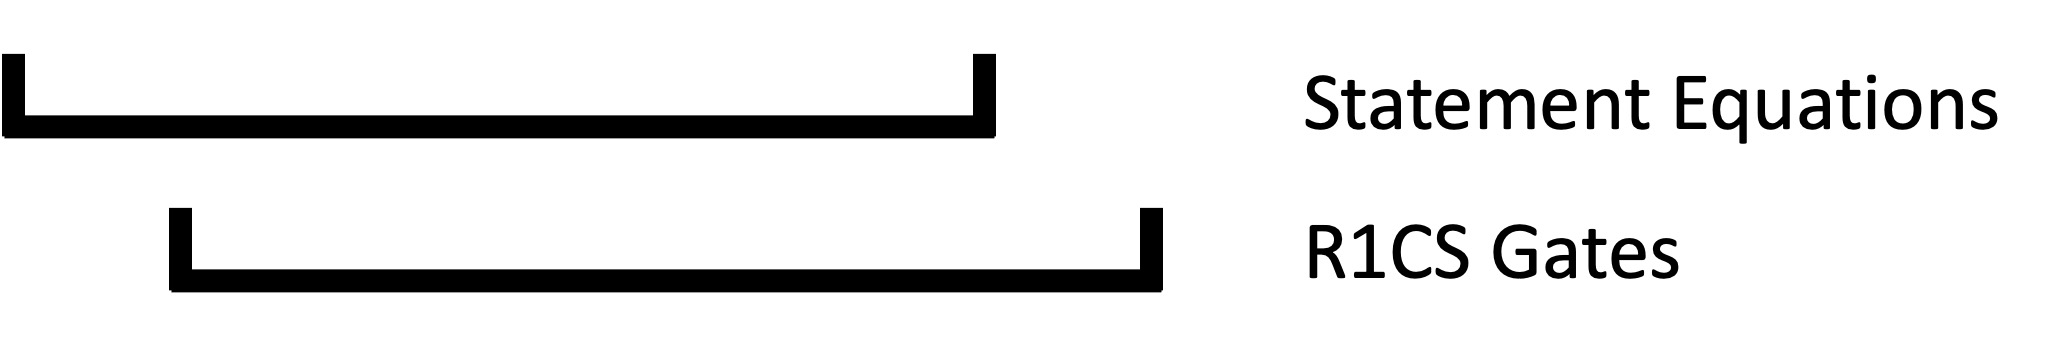
\includegraphics[width=2in]{ch-snarkprobe/figure/domain-a.jpg}
%   \vspace{-0.5cm}
  \caption{Upper Bound and Lower Bound Do Not Match}
  \label{subfig:snarkprobe-domaina}
\end{subfigure}
\hspace{0.7cm}
\vspace{0.5cm}
\begin{subfigure}{0.4\textwidth}
  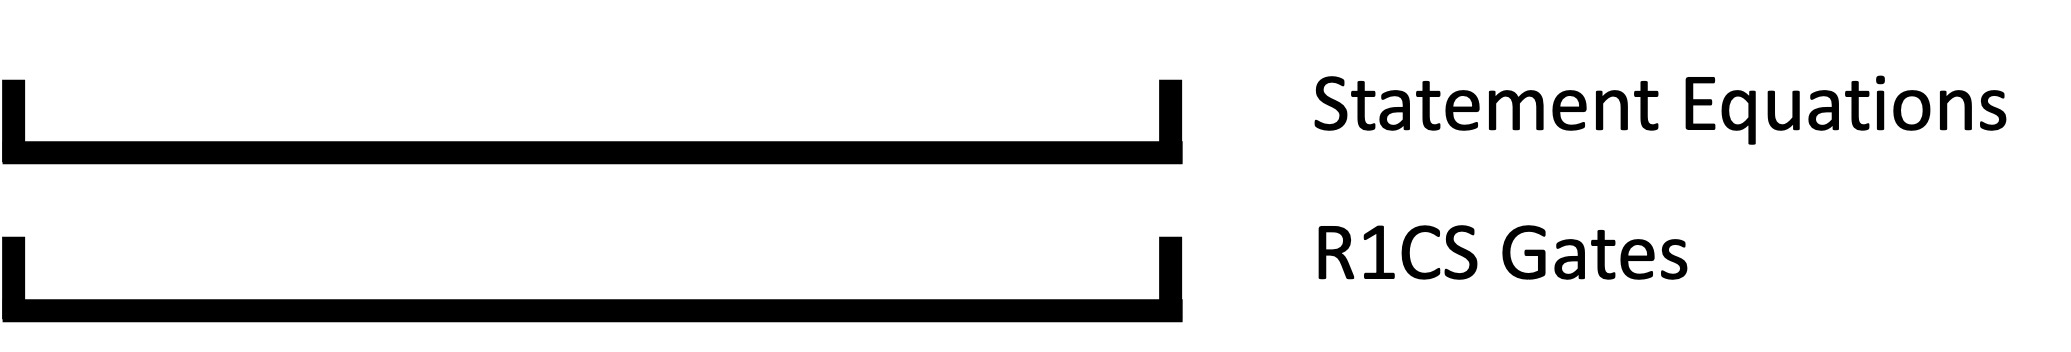
\includegraphics[width=2in]{ch-snarkprobe/figure/domain-b.jpg}
%   \vspace{-0.5cm}
  \caption{Upper Bound and Lower Bound Match}
  \label{subfig:snarkprobe-domainb}
\end{subfigure}
\begin{subfigure}{0.4\textwidth}
  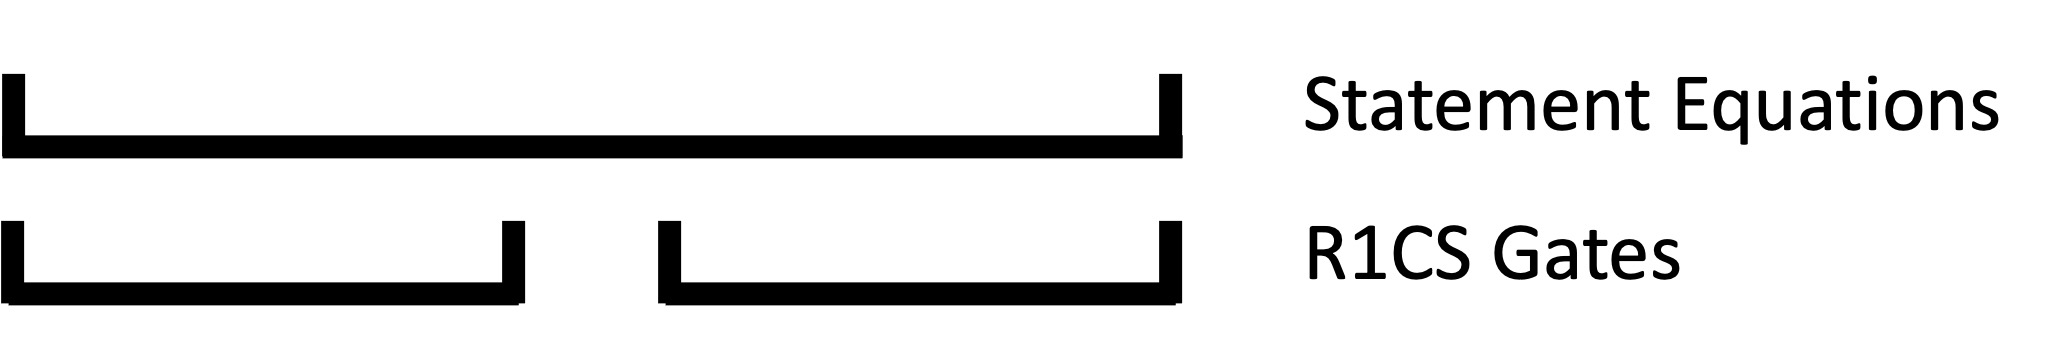
\includegraphics[width=2in]{ch-snarkprobe/figure/domain-c.jpg}
%   \vspace{-0.5cm}
  \caption{R1CS Gates Has Gap Between Bound}
  \label{subfig:snarkprobe-domainc}
\end{subfigure}
\hspace{0.7cm}
\begin{subfigure}{0.4\textwidth}
  
\includegraphics[width=2in]{ch-snarkprobe/figure/domain-d.jpg}
%   \vspace{-0.5cm}
  \caption{Statement Equations Has Gap Between Bound}
  \label{subfig:snarkprobe-domaind}
\end{subfigure}
\caption{Examples of Domain Comparison}
\label{fig:snarkprobe-domain}
%%\vspace{-3mm}
\end{figure}

%\newpage

%%%%%%%%%%

%\section{Comparison Between Standard Fuzzing and \SnarkFuzzer}
%
%\begin{figure}[h]
%\centering
%%\captionsetup{justification=centering}
%\begin{subfigure}{0.4\textwidth}
  %\includegraphics[width=3in]{imgs/fuzzing-a.jpg}
  %\vspace{-0.5cm}
  %\caption{Standard Fuzzing Test Procedure}
  %\label{subfig:snarkprobe-fuzzing1}
%\end{subfigure}
%\begin{subfigure}{0.4\textwidth}
  %\includegraphics[width=3in]{imgs/fuzzing-b.jpg}
  %\vspace{-0.5cm}
  %\caption{\SnarkFuzzer Procedure}
  %\label{subfig:snarkprobe-fuzzing2}
%\end{subfigure}
%\vspace{-0.2cm}
%\caption{Procedure Differences Between Standard Fuzzing Test and \SnarkFuzzer}
%\label{fig:snarkprobe-fuzzing}
%%%\vspace{-3mm}
%\end{figure}

%\newpage

%%%%%%%%%%

%\newpage

%%%%%%%%%%

%%%%%%%%%%

% \section{Additional Performance Results}
% \label{app:snarkprobe-additionalgraphs}

% \parhead{Performance of the \inputgenerator.}
% Unlike a mutation-based or generation-based fuzzer for an invalid matrix (which are very quick since they only require straightforward operations), generating a valid R1CS matrix with our generation-based fuzzer requires the SMT solver to produce a matrix based on the random witness array. Thus the processing time depends on the matrix size and random value(s) in the witness list, which generally results in a larger matrix taking longer to process.
% To validate this, we used our various fuzzers to produce matrices of varying sizes (remember that the rows represent the number of constraints and columns the number of variables). In Table \ref{tab:gen-invalid}, we present the processing time for each method (generally under one second for most methods), which confirms our general intuition.
% We also note that the \inputgenerator must compile the input matrix (proof) and source code into a binary program, which can require substantial time that is outside of our control.
% %Some \zksnark libraries may require longer compiling time, and we have no control to the library compiling time cost, which will increase our \inputgenerator total runtime.
% %\delete{ Although a larger matrix usually takes a longer time to generate, a ``smaller'' R1CS matrix may also require greater computational resources depending on the random numbers chosen in the witness and R1CS relations, as this can cause simplified relations in R1CS matrix and witness, thus requiring the SMT solver to take less time to calculate a valid R1CS matrix.\yuquan{Might need better explanation for this line?}  For example, we can see that matrix three and matrix seven in the 10 × 200 category only take roughly ten seconds to generate, which is similar to generating a matrix of size 20 × 40.} \fanyo{(summary)}

% %\begin{figure}[t]
%   %\centering
%   %%\captionsetup{justification=centering}
%   %\includegraphics[width=0.9\linewidth]{imgs/gen-invalid.jpg}
%   %\caption{Runtime of the \inputgenerator to produce R1CS matrices of different sizes.}
%   %\label{fig:snarkprobe-gen-invalid}
% %\end{figure}

% \begin{table}[h]
% %\captionsetup{justification=centering}
% \hspace*{0.15in}
% \begin{minipage}{\textwidth}
% \centering
% {\origfootnotesize
% \begin{tabular}{ll||c|c|c|c}
% \hline
% \multicolumn{2}{l||}{Matrix Size} & 5 × 10 & 20 × 40 & 50 × 100 & 50 × 200 \\ \hline\hline
% \multicolumn{1}{l||}{\multirow{2}{*}{}Generation Based} & Invalid Matrix & \textless{}0.01 & \textless{}0.01 & \textless{}0.01 & 0.02 \\ \cline{2-6}
% \multicolumn{1}{l||}{} & Valid Matrix & 0.16 & 2.06 & 23.02 & 51.27 \\ \hline
% \multicolumn{1}{l||}{\multirow{2}{*}{}Mutation Based} & Invalid Matrix & 0.38 & 0.49 & 0.65 & 0.77 \\ \cline{2-6}
% \multicolumn{1}{l||}{} & Valid Matrix & \textless{}0.01 & \textless{}0.01 & \textless{}0.01 & 0.02 \\ \hline
% \end{tabular}
% }
% \end{minipage}
% \caption{Runtime (in seconds) of the \inputgenerator to produce R1CS matrices of different sizes.}
% \label{tab:snarkprobe-gen-invalid}
% \vspace*{-14pt}
% \end{table}

% %%%%

% \parhead{Performance of the \branchmodel.}
% Next, we explore the coverage ability of the \branchmodel in terms of breadth, as well as how quickly we achieve a high percentage of branch coverage.  We ran 50 iterations of the \branchmodel with \libsnark, which covers more than 85\% of all branches.  We stopped our experiments after 50 iterations as \SnarkFuzzer did not reach any new branches over the previous 10 prior iterations.  Even with this, we note that after roughly 30 iterations we see the breadth of our coverage begin to taper off.
% A graph can be found in Figure \ref{fig:coverage}.
% %\fanyo{Even the \tool have covered most pf the branches in the target libraries, the fuzzer should not be stopped in order to generate more different inputs to test a same branch. The fuzzer should not be stopped until most of the branches have been tested for at least one time. As more inputs are generated, \tool has higher chance to find the potential issues in the target library or higher confidence to say (need a better word) that the target library is safe. }
% %There are a number of factors that can affect our coverage results. First, we can encounter situations where the generation-based fuzzer cannot produce enough diverse input sets to cover all branches, which is where the seeds of the mutation-based fuzzer can play an important role in coverage.  Second, \SnarkFuzzer allows a user to configure the proportion of matrices generated by each sub-fuzzing method, which can also affect the coverage result. In our experiment, we had the generation-based fuzzer produce 5\% invalid and 45\% valid matrices, and the mutation-based fuzzer produce 40\% invalid and 10\% valid matrices. Increasing the fuzzing time and/or adding extra seeds for the mutation-based fuzzer can improve the coverage of a target source library.

% \begin{figure}[h]
%   \centering
%   %\captionsetup{justification=centering}
%   
\includegraphics[width=0.70\linewidth]{imgs/coverage.jpg}
%   \vspace*{-10pt}
%   \caption{Percentage (breadth) of library coverage after a given number of iterations}
%   \label{fig:snarkprobe-coverage}
%   %\vspace*{-8pt}
% \end{figure}

% %%%%%%%%%%
